\section{Main contributions}\label{contributions}
The main contribution of this thesis is the theoretical foundation of a new approach to UI development that reduces development costs. A proof of concept of a UI framework that can be used by any UI developer demonstrates the major theoretical contributions.

\paragraph{Scope}
The scope of this thesis includes following artifacts:
\begin{itemize}
\item a hypermedia vocabulary and specification
\item implementations of two HTTP APIs using that hypermedia vocabulary
\item an evaluation of design languages
\item a proof of concept of a UI framework
\end{itemize}
The evaluation and creation of the hypermedia vocabulary is driven by the implementation of the HTTP APIs. The development of the HTTP APIs is driven by use cases that come from real world problems. The UI framework is then used to create client that can consume those two HTTP APIs which conform to a certain specification and make use of that hypermedia vocabulary.

\subsection{Methods}
This sections describe the methodological approach to achieve the items listed in the paragraph above.

\subsubsection{General approach}
The structure of this thesis consists of three parts.

\begin{enumerate}
\item The first part is concerned with research of hypermedia vocabularies and specifications and the evaluation of design languages. This includes research of the use of hypermedia, linked data and web components. The goal is to gather research results in order to base further work on top.
\item The second part defines two real-world use cases of web applications. By looking at the deficits of contemporary solutions for UI development we define design goals for the UI framework. We summarize the insights gained by implementing on HTTP API for each use case and by developing the UI framework. This part follows best practices from agile software development and thus contains two iterations. The goal is the implementation of a proof of concept UI framework and the two real-world use cases.
\item The last part evaluates the UI framework by analyzing its impact on software complexity. Furthermore we assess whether the design goals have been met and we give an outlook on future work in this context.
\end{enumerate}

\subsubsection{Use of scores}
In order to evaluate the UI framework and its concepts we are using two scoring systems. To asses whether goals have been met scores between 0 and 3 are used. To gauge how complexity has been effected we use scores between -3 and 3.

\begin{table}[]
  \begin{center}
    \begin{tabular}{|c|l|}
      \hline
      Score & Effect on goal \\
      \hline
      0 & Goal not met \\
      1 & Slight improvement towards goal \\
      2 & Goal mostly met \\
      3 & Goal completely fulfilled \\
      \hline
    \end{tabular}
    \caption{Scores to evaluate whether goals have been met}
  \end{center}
\end{table}

\begin{table}[]
  \begin{center}
    \begin{tabular}{|c|l|}
      \hline
      Score & Effect on complexity \\
      \hline
      -3 & Massive increase in complexity \\
      -2 & Increase in complexity \\
      -1 & Slight increase in complexity \\
      0 & No change in complexity \\
      1 & Slight decrease in complexity \\
      2 & Decrease in complexity \\
      3 & Massive decrease in complexity \\
      \hline
    \end{tabular}
    \caption{Scores to gauge the change in complexity}
  \end{center}
\end{table}

\subsubsection{Steps}
This section lists and describes the steps that we take in this thesis.

\paragraph{Conceptual analysis of user interfaces}
Before defining the use cases we analyze UIs on a conceptual level. By looking at typical usage patterns of UIs by end users we aim to describe the nature of UIs. The goal are insights which can be further used to define the requirements of the UI framework.

\paragraph{Hypermedia vocabulary and specification}
This section explores hypermedia vocabularies and specifications. By listing requirements that such a specification has to cover we either create our own hypermedia specification, use an existing one or mix bits and pieces of existing ones.

\paragraph{Evaluation of design languages and their implementations}
We evaluate popular design languages and their implementations. The UI generation is based on top of an existing design language so that best practices in design and presentation of UIs are respected.

\paragraph{Definition of major design goals}
Major design goals of the UI framework are directly influenced by non-functional requirements. We consider the broader scope of UI development in order to obtain those. This includes analysis of:

\begin{enumerate}
  \item the development process of UIs with web technologies
  \item contemporary frameworks and tools for UI development that enjoyed wide and rapid adoption
  \item contemporary frameworks and tools for UI development that failed
\end{enumerate}

By following what tools in \textbf{2} did right and avoiding the mistakes of tools in \textbf{3}, we define a set of design goals that the proof of concept should adhere to.

\paragraph{Specification of the proof of concept}
The section defines the artifact that can be used to create UIs. The proof of concept should demonstrate the viability of the thesis.

\paragraph{Definition of real world use cases}
By defining real world applications for the UI framework, we discover user roles and user stories.

\paragraph{Implementation of proof of concept driven by use cases}
The UI framework is developed incrementally use case by use case. The major design goals are respected. We expect to gain theoretical insights while implementing both the UI framework and the HTTP APIs.

\paragraph{Evaluation of design goals}
We analyze the design goals and whether they have been met. The design goals are not equally important, so they get a weight assigned. We assess each design goal qualitatively and assign a score between 0 and 3.

The mean of all scores is calculated to asses whether the design goals have been met.

\paragraph{Conclusion of approach to reduce development costs}
We break up software complexity into more specific types of complexities. Software complexity comprises Essential Complexity and Accidental Complexity according to Brooks. Essential Complexity has several causes on its own.

After identifying types of complexity, we asses how the UI framework affects them by assigning a score between -3 and 3.

\subsection{Conceptual analysis of user interfaces}
For a system to be useful, it has to interact with its environment. These interactions happen through multiple types of interfaces, which are used by two types of users. The users are either other systems or human users.
The interfaces for human users (user interfaces) have typical characteristics,
By observing the usage of a user interface by the user we can analyze the main characteristics. A typical scenario of UI usage is browsing a website. What does the user do while browsing a website? It is typically one of two things: he either reads or clicks.

\textbf{Reading} a website is equivalent to data \textbf{querying}. The user \textbf{querying} data

The usage of a UI by a user consists of either \textbf{reading} or \textbf{interacting}. In terms of systems we can call them \textbf{querying} or \textbf{interacting} respectively.
\begin{enumerate}
  \item Query: The user is able to retrieve information from the UI by looking at it
  \item Interacting: The user is able to interact with the UI
\end{enumerate}

The development of the UI framework is driven by the implementation of these two capabilities. Each of the use cases covers one of them.


\subsection{Hypermedia API specifications}
The goal is to pinpoint a specification among existing hypermedia API specifications. The real world uses cases will implement HTTP APIs that conform to this specification. The client that consumes such a hypermedia API is merely a console. This implies the client doesn't contain any knowledge about the API implementation, it is sufficient to know about the specification. \\ Following requirements have to be addressed by the chosen specification in some form:

\paragraph{Self documentation}
The API should provide its own documentation so the consumer doesn't have to use a third party tool.

\paragraph{Discoverability}
The consumer should be able to autonomously discover the data model of an API implementation.

\paragraph{Actions and Operations}
The specification should provide a concept on how to interact with it. Ideally the API publishes the data that is needed by the client to build action objects or operations that can be invoked.

\paragraph{Uses linked data}
Based on the discussion in section \ref{linkeddata} about the benefits of linked data this thesis assumes that linked data is the key concept to efficient UI development. In combination with the web component based rendering discussed in section \ref{webcomponents} it allows the UI developer to think in terms of components and data.

\subsubsection{Hydra}
It is remarkable that at the time of writing this thesis only one specification exists that satisfies the requirements stated above.

\href{http://www.hydra-cg.com/}{Hydra} is a lightweight specification to create hypermedia-driven Web APIs. By specifying a number of concepts commonly used in Web APIs it enables the creation of generic API clients \citep{hydraspecs}. At the time of writing the Hydra specification exists only as an unofficial draft.

The two major benefits of APIs supporting hypermedia are \textbf{discoverability} and \textbf{self documentation}. \\
\paragraph{Discoverability} Discoverability is given by the RESTful nature of a hypermedia API. The API provides an entry point and each resource describes the means to fetch other resources. The client is able to traverse the API by sending requests to the server, there is no additional documentation needed. All paths and resources that are interesting to the client he can reach.

\paragraph{Self documentation}
A hypermedia API documents itself by providing meta data along the actual data. There is no need for other documentation tools because the hypermedia vocabulary provides primitives for built-in documentation.
Hypermedia APIs can use the same data model for generating built-in documentations as the actual API uses. These documentations are more likely be up-to-date and the maintenance cost is low due to automation.

Every Hydra resource has a documentation attached to it. By default the response contains the \textbf{Link} header of the URL to the documentation.

\paragraph{Collections, partial views and pagination}
In the world of Hydra there are conceptually only things and lists of things. A further nesting doesn't exist and it is not possible a list of lists of things.
Hydra calls a list of things \textbf{collection}, which can have things as members. There is the concept of a \textbf{partial view} on a collection. This gives the client the ability to fetch a subset of a collection. That partial view can be controlled by client initiated \textbf{pagination}. The client provides a limit and an offset when requesting a collection in order to initiate pagination.

\paragraph{Operations}
In order to interact with the server a client has to know which operations the server supports. Hydra supports this concept by exposing all information necessary to build and invoke operations. This allows any client that understands Hydra to interact with a Hydra API without any prior knowledge about the concrete API implementation. This part is not fully specified yet at the time of writing. The author had to directly communicate with Hydra core members and reverse engineer tools in the Hydra ecosystem in order to understand how Hydra operations are supposed to work.

\subsection{Design languages}
A design language or design vocabulary is an overarching scheme or style that guides the design of a complement of products or architectural settings. Designers wishing to give their suite of products a unique but consistent look and feel define a design language for it, which can describe choices for design aspects such as materials, colour schemes, shapes, patterns, textures, or layouts. They then follow the scheme in the design of each object in the suite. \citep{designlanguage}

For this thesis the benefit of the use of a design language is the consistent look and feel of UIs that \textbf{are composed of a set of small components}. Additionally it frees the UI developer from cumbersome work like making sure that the UI is responsive and behaves well on various screen sizes. UI developers can communicate and think in a higher level of abstraction by omitting implementation details that are taken care of by design language implementations. As an example, it allows thinking about \textbf{small buttons horizontally next to each other} instead of considering the actual implementation of those horizontally aligned buttons.

The major design languages are built on top of years of research in Human-computer interaction. Evaluation of the theoretical foundation is not in the scope of this thesis, it can however benefit off the implementations and tools.

\subsubsection{Design language implementations}
The UI framework will consume React components and it will internally use React as well. The only requirement to the design language implementation is the use of React.

\paragraph{Material Design}
Material Design was developed at Google in 2014. Initially it was used in Google's own mobile apps and in the mobile OS Android. In order to offer a consistent user experience across all products Google makes use of it in web products as well.

The React implementation of Material Design is called Material UI. It bottles up the UX best practices and provides them in form of React components. \\ After implementing a simple form with three text fields and a button we conclude that Material UI is too heavyweight. It is not always obvious how to configure components, especially big ones. The main contribution of Material Design and Material UI are best practices in UX. This reaches beyond simple forms and visualization of lists. Material Design dictates the look and feel of menus and navigations. \\ The UI Framework requires a lower level design language implementation that doesn't make assumptions or rules about how larger components look or behave.

\paragraph{Semantic UI}
Semantic empowers designers and developers by creating a shared vocabulary for UI. \citep{semanticui} This thesis explores the benefits of shared vocabularies in HTTP APIs. Semantic UI is not as widely adopted as Material Design, but there exists a React implementation and the level of abstraction fights the use case of generically rendering forms and navigations.

\begin{figure}[!htb]
  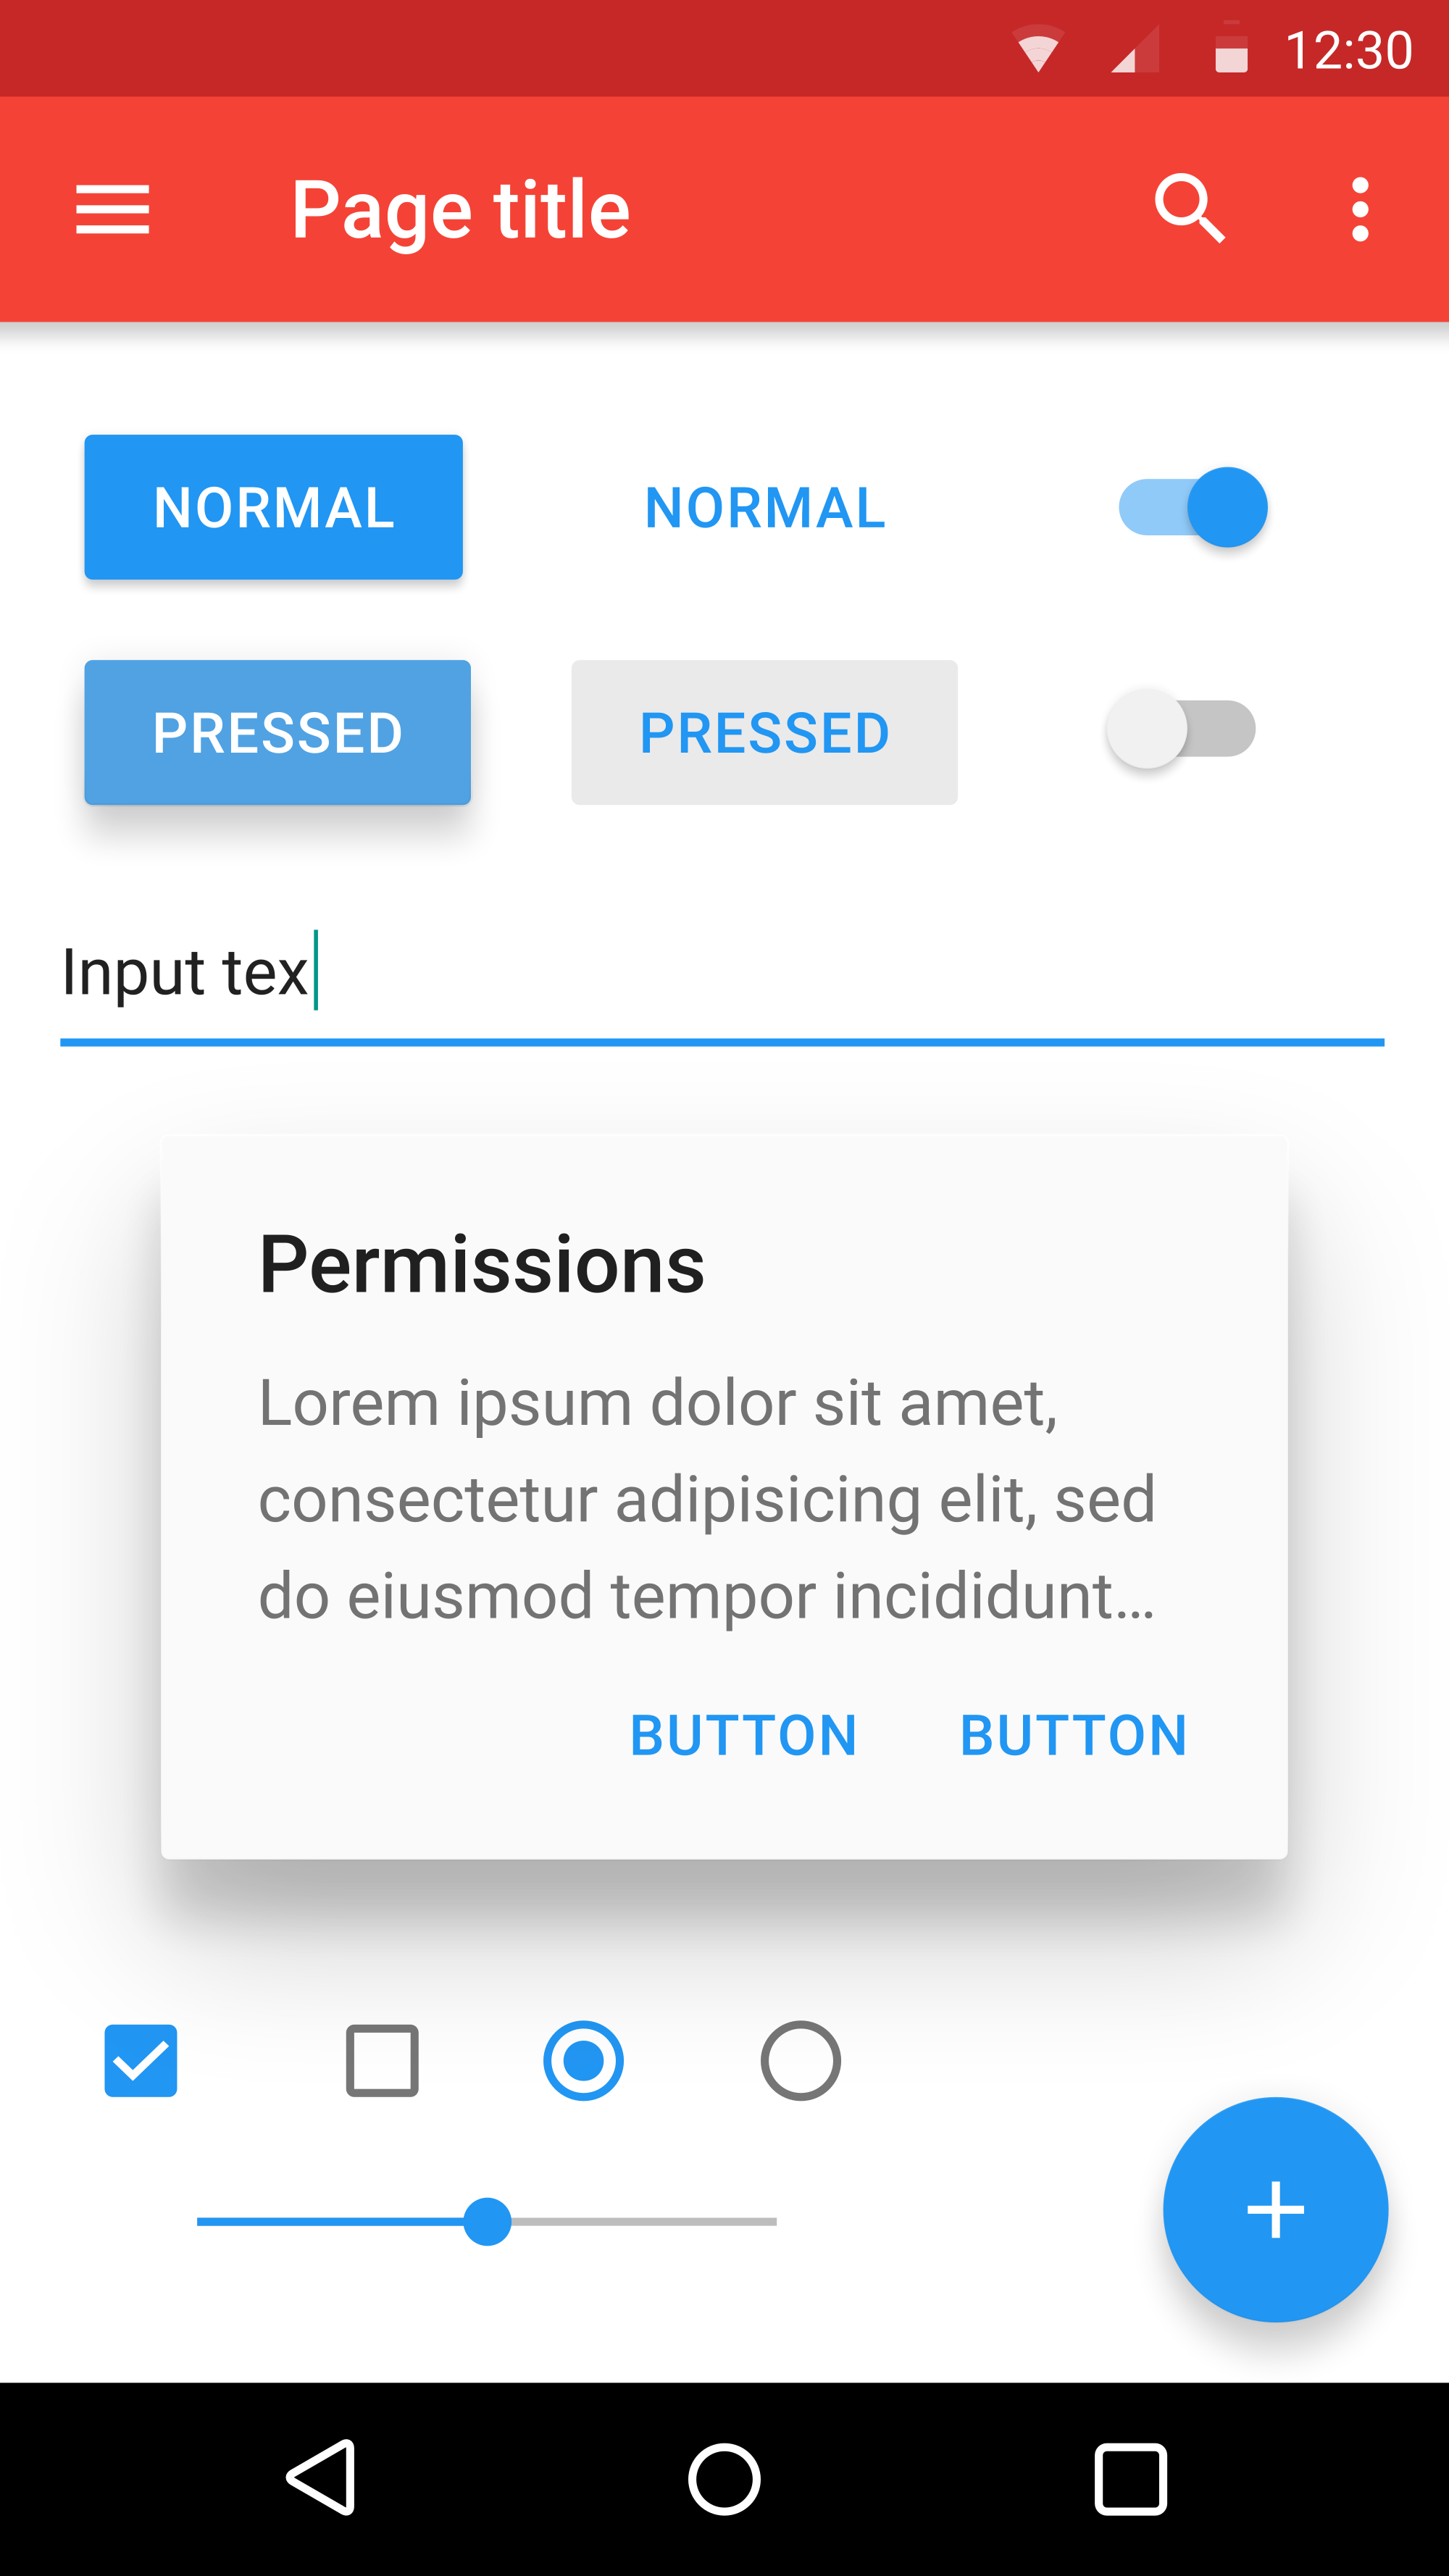
\includegraphics[width=150pt]
    {images/materialdesign.png}
  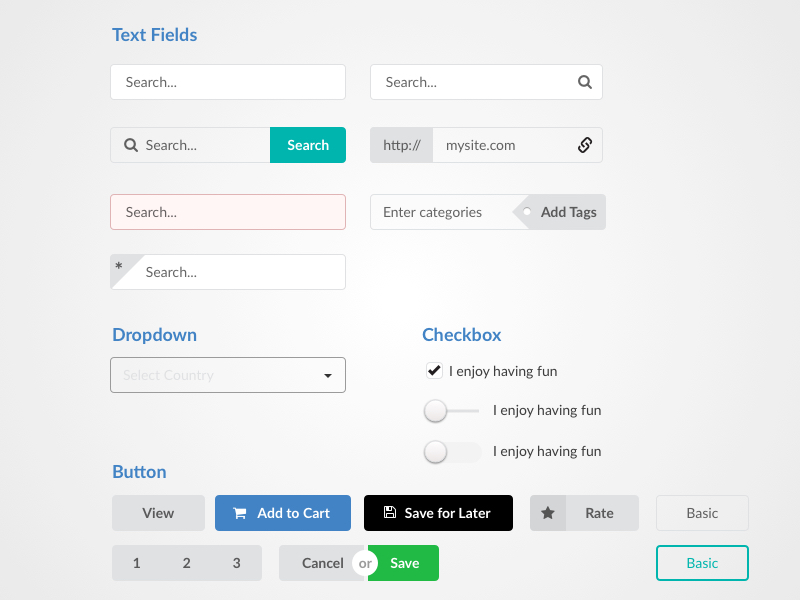
\includegraphics[width=320pt]
    {images/semanticui.jpg}
  \caption{Material Design on a mobile device (left) and Semantic UI components (right). (Source: https://wikipedia.org, https://www.sketchappsources.com/)}
\end{figure}

We pick Semantic UI and its React implementation.

\subsection{Design goals}
Following design goals should be met by the UI framework. For each design goal we discuss the goal itself, why and how we intend to meet it and how it can be measured.
The goals are partly derived by analyzing the deficits of contemporary tools to enhance UI and web development.

\subsubsection{Play nicely with others}
As discussed in section \ref{graphql} the fact that GraphQL doesn't play well with other is one of its major weaknesses. Playing nicely with others is the most important design goal of the UI framework because it allows to reuse and build on top of existing research and work.
It is important to respect standards and stay compatible with existing tooling. This design goal drove the choice of JSON-LD as serialization format for linked data.

We acknowledge the widespread use of HTTP and JSON as data exchange format and achieve this design goal by conforming to web standards and \textbf{extending} existing tooling. JSON-LD allows us to stay compatible with all tools consuming and producing JSON.

This design goal can be quantified by analyzing each component of the UI framework and determine whether the technologies, protocols, languages and tools for that component are either formally standardized or a defacto standard.

\subsubsection{Straightforward upgrade path}
In order to help the adoption of the UI framework it is important to show a clear upgrade path and to keep the friction at a minimum.

This can be achieved by \textbf{extending} existing standards, keep breaking changes at a minimum and with good documentation. Playing nicely with others helps to reach this design goal as well.

This design goal can be quantified by measuring or estimating the effort that needs to be spent to upgrade a conventional API to the suggested hypermedia API.

\subsubsection{Customizability}
While providing sane defaults, the UI framework should be customizable. There should be no limitations imposed in terms of what UIs can be drawn.

We want to achieve this goal be allowing the UI developer to override the sane defaults. The UI developer can decide to completely ignore the linked data aspect and consume the HTTP API in a traditional way by hard coding knowledge into the client. The use of React as UI library allows the UI developer to pull in external React components.

This design goal is met if all possible UIs that can be drawn with conventional tools can be drawn using the UI framework. By allowing the UI developer to consume the hypermedia API as conventional API this goal is met.

\subsubsection{Developer ergonomics}
The UI developer should be able to use the UI framework with spending minimal effort on learning.

This goal can be achieved by choosing a widely used platform that has a striving open source community. It is important that there is an open source community working on that platform because a wide adoption behind closed doors is less likely to improve developer ergonomics.
A big market share of the platform increases the chances that the developer is already familiar with it. The tooling of these platforms tends to be polished and battle tested. The developer is less likely to get stuck because of some edge case issues.

An established and widely adopted platform is Node and the NPM (Node Package Manager) ecosystem. This is the platform that we choose to develop the UI framework in.

\subsection{Proof of concept of UI Framework}\label{proofofconcept}
We define two real-world use cases that cover the two main capabilities of \textbf{rendering data} and \textbf{user interaction}. Each of those use cases are split up into user stories that can be implemented separately. This ensures that the design goals are met and all user roles are considered.

The proof of concept of the UI Framework consists of following components:

\paragraph{Hydra client}
The Hydra client is a wrapper around the Hydra HTTP API. It takes care of serializing Hydra resources, fetching Hydra documentation and invoking operations. The value it provides to us is mainly developer ergonomics. The most complete Hydra client is called Alcaeus which we are using as a part of the UI Framework.

\paragraph{Infrastructure}
The infrastructure allows UI developers to plug in their own components as renderers, it fetches data from the server using the Hydra client and it applies the renderers by providing them the data returned by the Hydra client. This component is the glue - it knows all other components.

\paragraph{JSON-LD Renderer}
The JSON-LD renderer is one of the two renderers that ship be default with the UI Framework. It's only purpose is to render the JSON-LD response from the server. Rendering JSON-LD is equivalent to rendering tree like data.

\paragraph{Hydra Renderer}
The Hydra renderer is the second renderer that ships with the UI Framework. It builds on top of the JSON-LD renderer and it renders root resources, collections, links and operations. The Hydra Renderer creates a UI on top of a Hydra API which a user can use to interact. That UI is not optimized for efficiency because there is no domain knowledge involved.

\paragraph{Domain Renderers}
This component describes the set of renderers are contributed by the UI developer. They contain domain knowledge and are only valid for certain data types. As discussed in section \ref{uidevelopmenttoday} contemporary clients and the web UIs they include are tightly coupled to HTTP APIs. The reason is the hard coded knowledge in the UIs about the domain models and rules. \\
The Domain Renderers render linked data instead of any data. This means the linked data provides its own context, the UI developer doesn't hard code assumptions about the data model of the HTTP API - only about the linked data. \\
A React component and a linked data type constitute one domain specific renderer. The open-world philosophy of linked data encourages reuse across company, department and team boundaries. Domain renderers can be shared together with vocabulary since they are not coupled to data models \textbf{but to linked data vocabularies}.

\paragraph{Semantic UI}
Semantic UI is a set of reusable React components that constitutes the bottled up best practices of UI and UUX.

\begin{figure}[!htb]
  \center{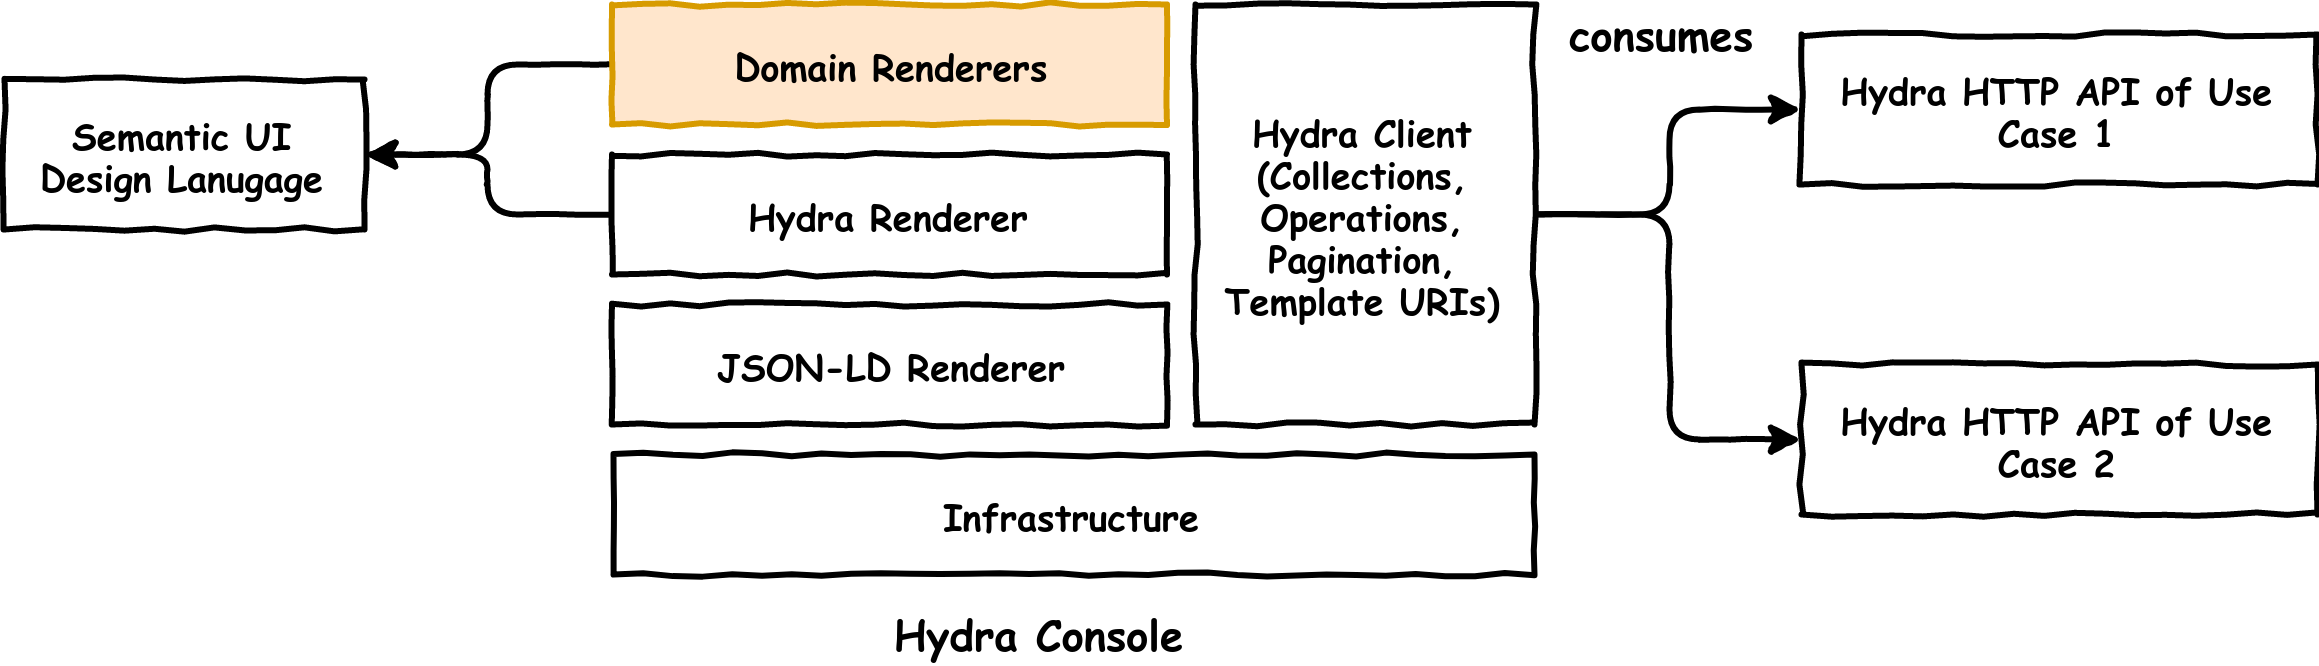
\includegraphics[width=400pt]
    {images/ui-framework-architecture.png}}
  \caption{The architecture of the proof of concept of the UI Framework.}
\end{figure}

\subsection{Use Case 1: Apartment}
For the user to be able to query data the UI has to render it.

The first use case describes a scenario in home automation. Several thermometers in several rooms in an apartment send the current temperature to a server. The goal is to develop a UI that displays apartments, rooms, and thermometers and temperatures in a sensible manner.

\begin{figure}[!htb]
  \center{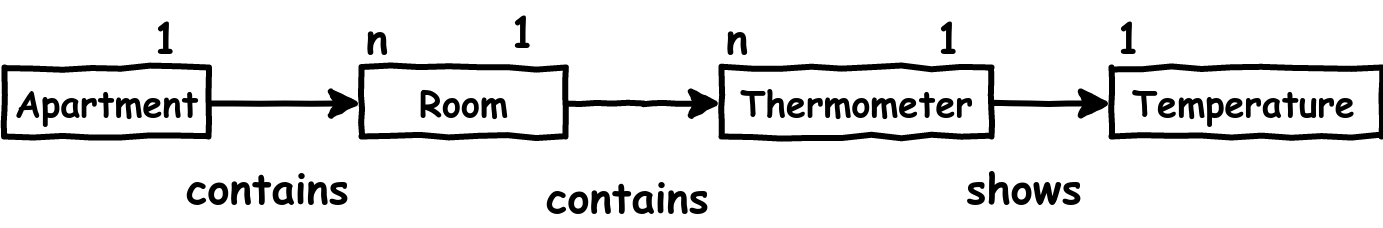
\includegraphics[width=100pt]
    {images/iot.png}}
  \caption{Data model of the apartment use case.}
\end{figure}

\begin{table}
  \begin{center}
    \begin{tabular}{ |c|l| }
      \hline
      ID & Story title \\
      \hline
      S01 & As landlord I want to overview my apartments \\
      S02 & As landlord I want to overview all rooms of an apartment \\
      S03 & As landlord I want to overview thermometers of room \\
      S04 & As landlord I want to overview the measurement data of a thermometer \\
      S05 & As UI developer I want to present all available data without spending any development time \\
      S06 & As UI developer I want to be able to customize the UI in order to improve it incrementally \\
      \hline
    \end{tabular}
    \caption{User stories of a client that consumes a home automation API}
    \label{tab:usecase1}
  \end{center}
\end{table}

\subsubsection{Hydra Collection rendering}
Due to the data model the API exposes a collection of apartments, rooms and thermometers. Every Hydra API has an entry point and a set of root collections. These collections can be used as starting point to discover the API.

Hydra has native support for collections by using the property \lstinline{http://www.w3.org/ns/hydra/core#member}.

\lstset{language=JSON}
\begin{lstlisting}[caption=Data of /rooms as Hydra collection.]
  {
    "@context": "http://localhost:3000/iot/contexts/Room",
    "@id": "http://localhost:3000/iot/rooms",
    "@type": "Collection",
    "totalItems": 6,
    "member": [
      {
        "@id": "http://localhost:3000/iot/rooms/0",
        "@type": "https://schema.org/Room",
        "amenityFeature": "Kitchen",
        "containsPlace": [],
        "containedInPlace": "http://localhost:3000/iot/apartments/0",
        "geo": {...}
      },
      {
        "@id": "http://localhost:3000/iot/rooms/1",
        "@type": "https://schema.org/Room",
        "amenityFeature": "Laundry Storage",
        "containedInPlace": "http://localhost:3000/iot/apartments/0",
        "geo": {...}
      },
      ...
    ]
  }
\end{lstlisting}

Each member of this collection is of type \lstinline{https://schema.org/Room}. The properties can be looked up by following the URL of the type. Given every member of the collection is of the same type, we can implement a generic renderer that looks up the properties of the member type and renders the collection as a table.

\begin{figure}[!htb]
  \center{\includegraphics[width=500pt]
    {images/hydra-collection-rooms.png}}
  \caption{Generic table renderer applied on root collections.}
\end{figure}

The \lstinline{@id}s are rendered as links so that the API can be traversed by looking up resources and collections of resources.

\subsubsection{Plugin mechanism}
As shown in section \ref{proofofconcept} the architecture of the UI Framework support custom renderers as main mechanism to override default behavior. The UI developer starts out with the default set of renderers that can render arbitrary JSON-LD data and data coming from a Hydra API. \\
The fact that the API returns linked data benefits this customization process. The UI developer only cares about how to render \textbf{certain data types}. In our use case he might be concerned with rendering the data type \lstinline{Temperature}.

We demonstrate data rendering using the room called \textbf{Entrance}. The trivial JSON-LD renderer colors property keys red, properties that represent relationships blue and it renders \lstinline{@id}s as hyperlinks.

\begin{figure}[!htb]
  \center{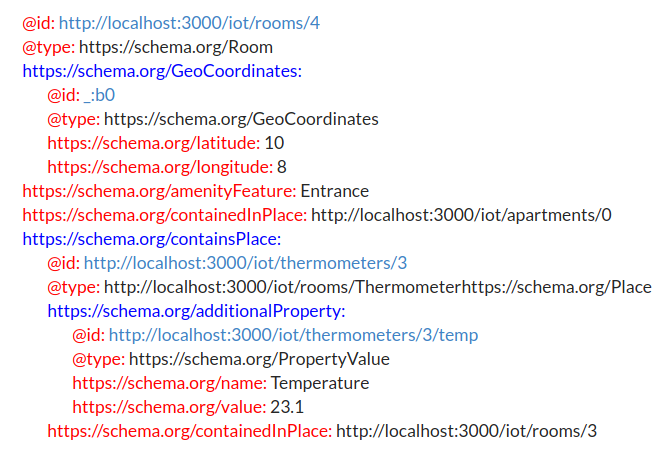
\includegraphics[width=380pt]
    {images/json-ld-renderer.png}}
  \caption{JSON-LD renderer applied on the data of /rooms/4.}
\end{figure}

This room contains a list of things of type \lstinline{Thermometer} and \lstinline{https://schema.org/Place}. The thermometer as a custom \lstinline{https://schema.org/additionalProperty} that as the name \textbf{Temperature} and a numeric value. \\ This is not straightforward to see as the JSON-LD is visually noisy. By applying a custom renderer to \lstinline{https://schema.org/additionalProperty} we render the temperature in one line with an icon indicating whether the temperature is hot or cold. This however requires domain knowledge since these differentiation holds only true in this context of room temperatures.

Considering the UI developer's workflow, the UI Framework expects a React component that takes the data of the \lstinline{https://schema.org/additionalProperty} and returns markup. The renderer that can be registered in the UI Framework comprises of a unique id, a name, a React component and a type. The type is used by the rendering infrastructure to determine which renderers to apply on what part of the server response.

\lstset{language=JSON}
\begin{lstlisting}[caption=Renderer configuration that the developer provides.]
  {
    id: "thermometer",
    name: "Thermometer",
    comp: (data) => <Thermometer/>,
    type: "http://localhost:3000/iot/apartments/Thermometer"
  }
\end{lstlisting}

\begin{figure}[!htb]
  \center{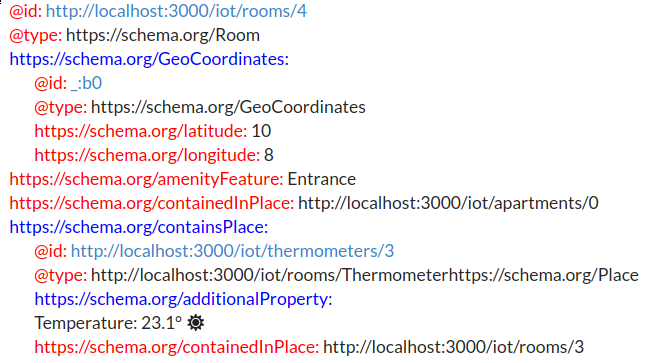
\includegraphics[width=380pt]
    {images/temperature-renderer.png}}
  \caption{The temperature renderer is applied on \lstinline{additionalProperty}. on top of the JSON-LD renderer.}
  \label{fig:temperature}
\end{figure}

It is noteworthy that renderer compose by stacking them on each other. As shown in figure \ref{fig:temperature} the temperature renderer works on top the JSON-LD renderer.

\subsubsection{Domain rendering}
Both the JSON-LD renderer and the Hydra renderer come with the UI Framework preconfigured. Internally both are registered using the plugin mechanism. Activating both renderers leads to a UI that is \textbf{correct} \footnote{Here we use the term \textbf{correct} in the sense of correct data rendering - the UI doesn't show wrong or non-existing data and it shows all of the response data} and the user is able to navigate through the API using hyperlinks. This rendering setup is decoupled from the API implementation, the only requirement it has is the conformity to Hydra.

In order to leverage domain information for visualizing data the UI developer has to provide custom components that contain domain knowledge. We demonstrate domain rendering by looking at one apartment.

\begin{figure}[!htb]
  \center{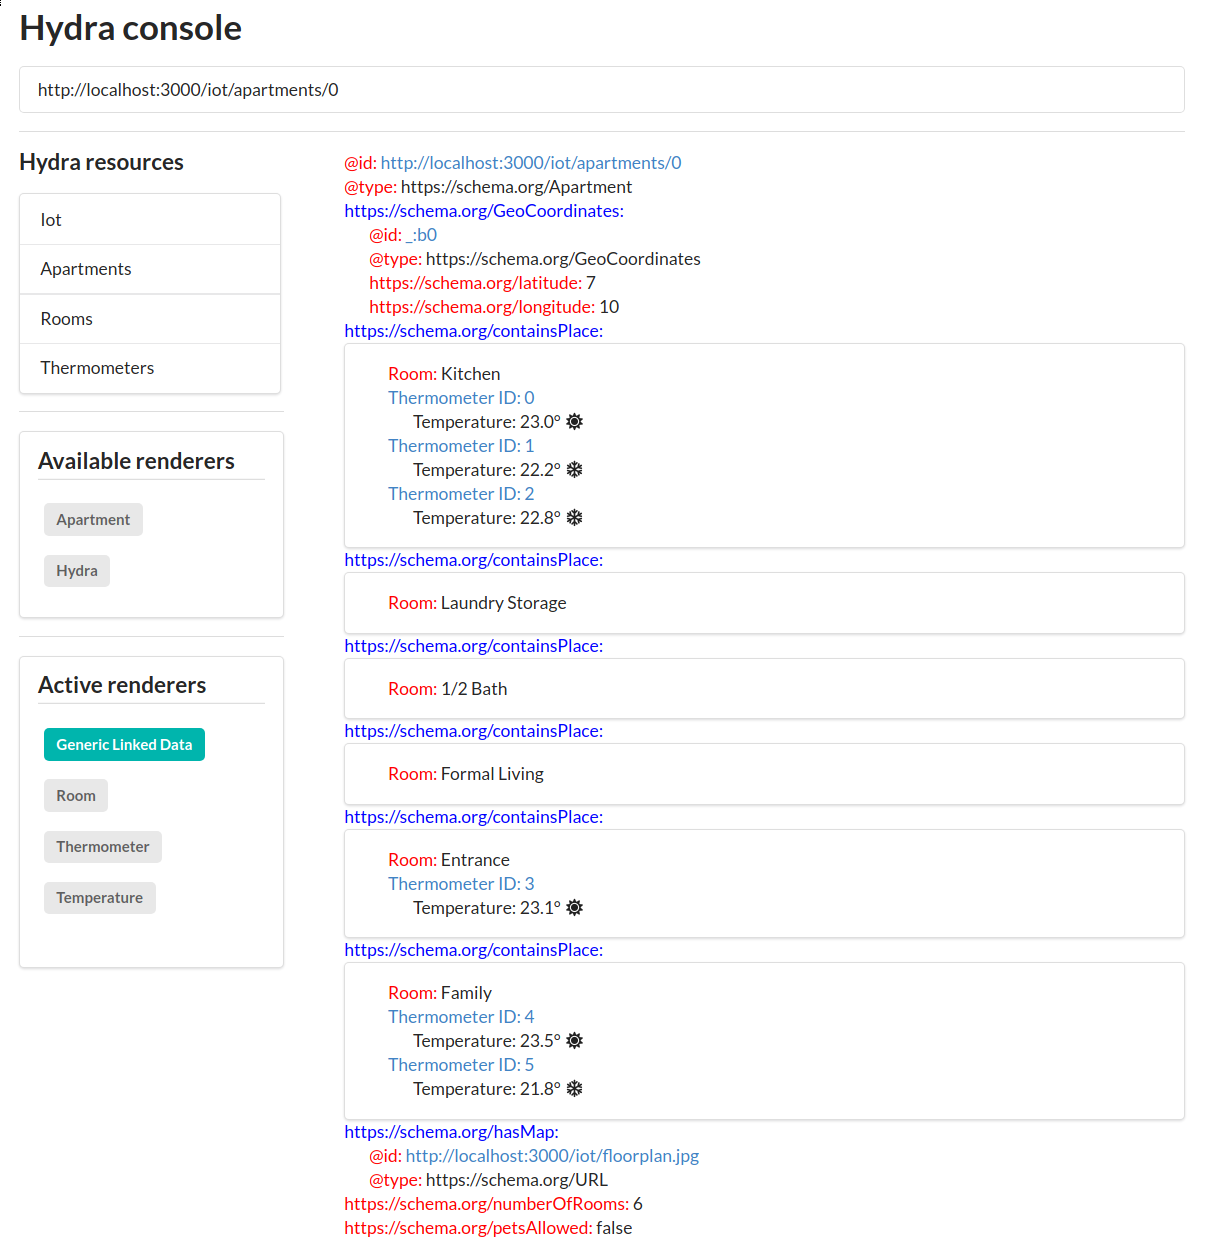
\includegraphics[width=500pt]
    {images/apartment-renderer.png}}
  \caption{Apartment data with applied renderers: JSON-LD, Thermometer, Temperature, Room.}
\end{figure}

The thermometer renderer removes some noise by compacting the thermometer data. The room renderer removes some properties that are not important in this context and it draws a box around the room so rooms are easier to distinguish. This list view provides all information to the landlord that he cares about. \\ Places and containment relationships of places can be visualized in a more intuitive way.

\paragraph{Floorplan}
The apartment has a property called \lstinline{https://schema.org/hasMap}.

\lstset{language=JSON}
\begin{lstlisting}[caption=The \lstinline{hasMap} property of apartment /apartments/0.]
...
  "hasMap": {
  "@type": "https://schema.org/URL",
  "@id": "http://localhost:3000/iot/floorplan.jpg"
}
...
\end{lstlisting}

This property has a link to an image representing the floor plan of the apartment.

\paragraph{Geo coordinates}
All things of type \lstinline{https://schema.org/Apartment} and \lstinline{https://schema.org/Room} can have a \lstinline{geo} property.

\lstset{language=JSON}
\begin{lstlisting}[caption=The \lstinline{https://schema.org/geo} property of apartment /apartments/0.]
...
  "geo": {
    "@type": "https://schema.org/GeoCoordinates",
    "longitude": 10,
    "latitude": 7
  }
...
\end{lstlisting}

This property contains the longitude and latitude coordinates of the center of the place.

Both properties \lstinline{https://schema.org/hasMap} and \lstinline{https://schema.org/geo} are defined on the type \lstinline{https://schema.org/Place}. \lstinline{https://schema.org/Apartment} is a subtype of \lstinline{https://schema.org/Place} in the schema.org hierarchy, so our apartment renderer has to expect the existence of those properties.

By leveraging coordinates of the places and the floor plan of the apartment we use domain knowledge to implement a renderer that provides additional value to the landlord. By rendering the rooms on the floor plan the landlord can grasp the locations of thermometers in a more natural way.

\begin{figure}[!htb]
  \center{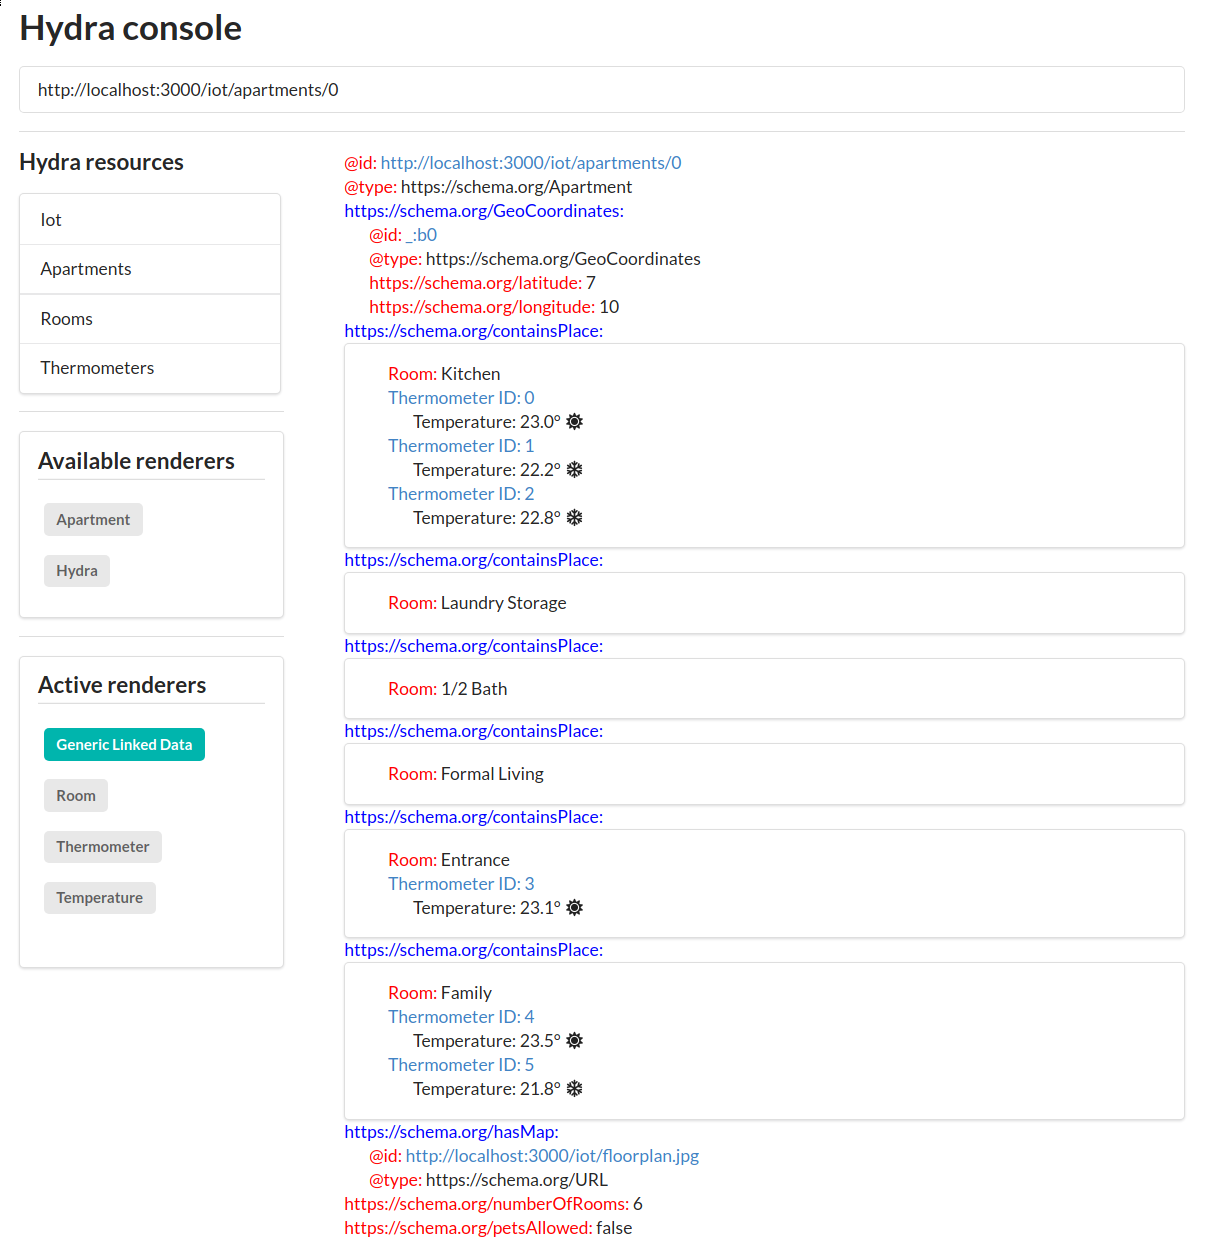
\includegraphics[width=500pt]
    {images/apartment-renderer.png}}
  \caption{Apartment data with applied renderers: JSON-LD, Thermometer, Temperature, Room, Apartment, BoldFont.}
\end{figure}

It is noteworthy that a set of renderers can be active at the same time. Whenever the rendering infrastructure encounters a data type that has a registered renderer it will apply it. In this example Hydra collections are still rendered as tables if the landlord opens the collection of rooms or thermometers.

\subsection{Verification of user stories}
In this section we verify that the user stories listed in table \ref{tab:usecase1} are fulfilled by either accepting or declining them.

\begin{table}
  \begin{center}
    \begin{tabular}{ |c|l| }
      \hline
      ID & Accepting/Declining \\
      \hline
      S01 & Accepting: The landlord can overview the apartments \\
      S02 & Accepting: The landlord can list all rooms of an apartment \\
      S03 & Accepting: The landlord can list all thermometers of a rooms \\
      S04 & Accepting: The landlord can see the temperature reported by a thermometer \\
      S05 & Accepting: The UI developer uses the default renderers to render a correct UI \\
      S06 & Accepting: The UI developer can register custom renderers to improve the UI incrementally \\
      \hline
    \end{tabular}
    \caption{All user stories are fulfilled and the first use case is implemented.}
  \end{center}
\end{table}

\subsection{Use Case 2: Kanban Board}

\begin{figure}[!htb]
  \center{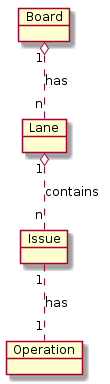
\includegraphics[width=100pt]
    {images/kanban.png}}
  \caption{Data model of the home automation use case.}
\end{figure}

\begin{table}
  \begin{center}
    \begin{tabular}{ |c|l| }
      \hline
      ID & Story title \\
      \hline
      S01 & As project manager I want to overview all projects \\
      S02 & As project manager I want to overview all issues of a project \\
      S03 & As project manager I want to see the status of an issue \\
      S04 & As project manager I want to change the status of an issue \\
      S05 & As project manager I want to create new issues \\
      S06 & As project manager I want to remove issues \\
      S07 & As UI developer I want to present all available data without spending time \\
      S08 & As UI developer I want to be able to customize the UI in order to improve it incrementally \\
      S09 & As UI developer I want to have an interactive UI without spending time \\
      \hline
    \end{tabular}
    \caption{User stories of a simple software project management tool}
  \end{center}
\end{table}

\begin{figure}[!htb]
  \center{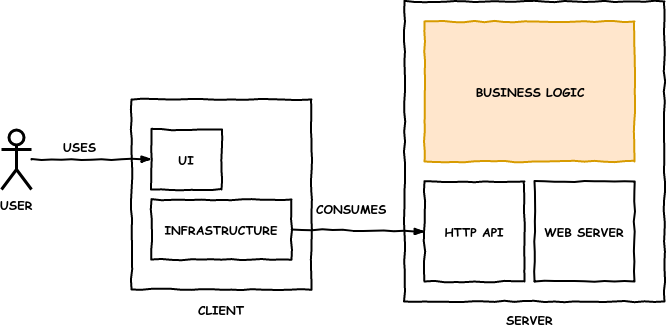
\includegraphics[width=380pt]
    {images/ui-dev.png}}
  \caption{Solely the server contains business logic.}
\end{figure}

\begin{figure}[!htb]
  \center{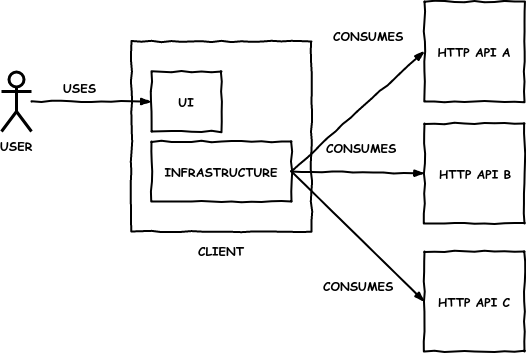
\includegraphics[width=380pt]
    {images/client-instances.png}}
  \caption{The client is decoupled from any API and is able to consume different APIs.}
\end{figure}

\begin{figure}[!htb]
  \center{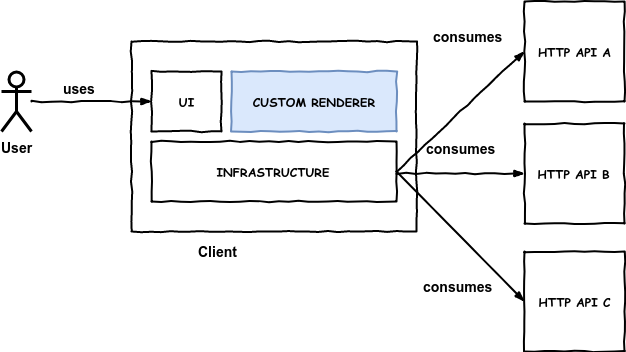
\includegraphics[width=380pt]
    {images/ui-dev-custom-renderer.png}}
  \caption{Custom renderers provide the ability to render linked data types. By avoiding hard coding business logic into the client the coupling to the server is still lose.}
\end{figure}

\subsubsection{Task based computing}

TODO

\subsubsection{User interaction}

TODO three types of operations:

inline operations
supported operations for all of the resource's types
supported operations for the supported property, where the resource is an object of said property

\subsubsection{CQRS}
